% Asset ID: AS2StatisticalSamplingTIKZ-004
% Unit: AS2 Applied Mathematics
% Topic: AS2-SAMP Statistical sampling
% Purpose: Types of data classification tree
% Source: Supplied Data Collection PDF page 20 and transcript Data Collection 5
% Linked LO IDs: AS2-SAMP-LO001

\documentclass[tikz,border=8pt]{standalone}
\usetikzlibrary{positioning,arrows.meta}
\begin{document}
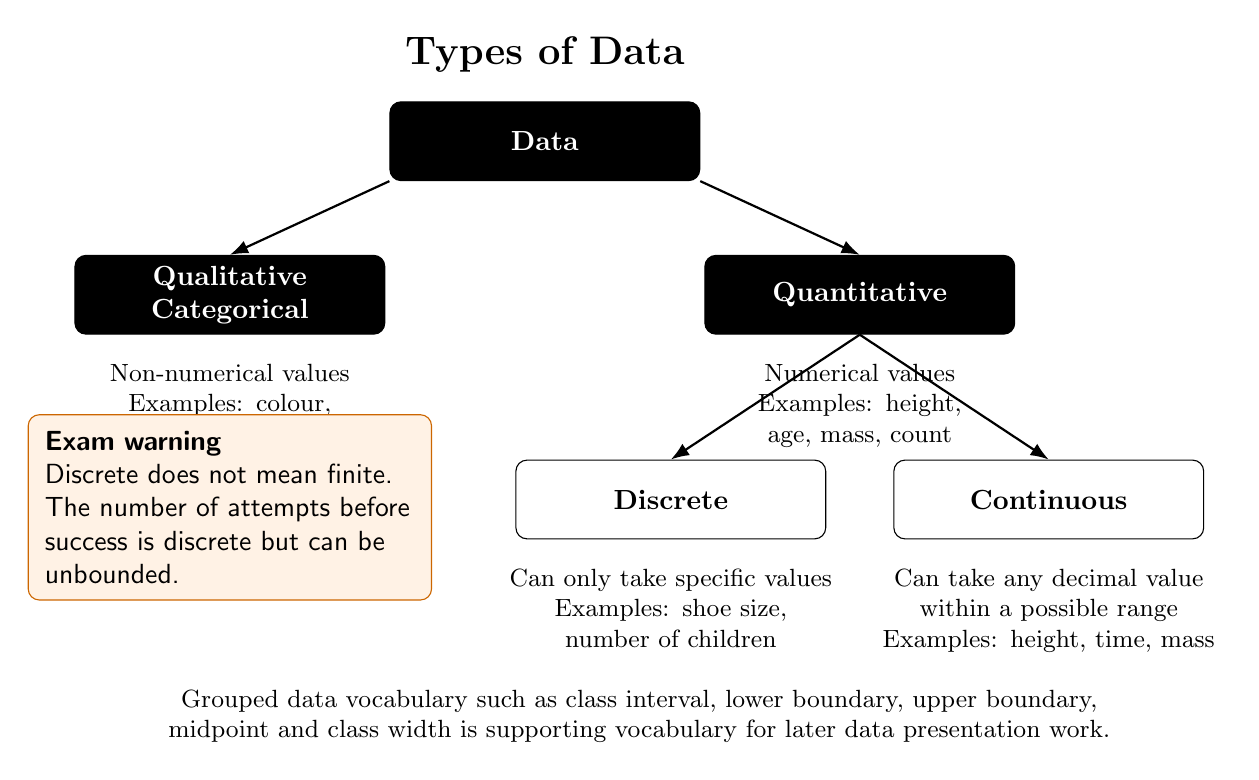
\begin{tikzpicture}[
  font=\sffamily,
  nodebox/.style={draw=black,fill=black,text=white,rounded corners=4pt,align=center,font=\bfseries,text width=3.7cm,minimum height=1.0cm},
  lightbox/.style={draw=black,fill=white,rounded corners=4pt,align=center,font=\bfseries,text width=3.7cm,minimum height=1.0cm},
  note/.style={align=center,text width=4.4cm,font=\small},
  warn/.style={draw=orange!80!black,fill=orange!10,rounded corners=4pt,align=left,text width=4.7cm,inner sep=6pt},
  arrow/.style={-Latex,thick}
]
\node[font=\bfseries\Large] at (0,4.3) {Types of Data};
\node[nodebox] (data) at (0,3.2) {Data};
\node[nodebox] (qual) at (-4.0,1.25) {Qualitative\\Categorical};
\node[nodebox] (quant) at (4.0,1.25) {Quantitative};
\draw[arrow] (data.south west) -- (qual.north);
\draw[arrow] (data.south east) -- (quant.north);
\node[note,below=0.25cm of qual] {Non-numerical values\\Examples: colour, species, type};
\node[note,below=0.25cm of quant] {Numerical values\\Examples: height, age, mass, count};
\node[lightbox] (disc) at (1.6,-1.35) {Discrete};
\node[lightbox] (cont) at (6.4,-1.35) {Continuous};
\draw[arrow] (quant.south) -- (disc.north);
\draw[arrow] (quant.south) -- (cont.north);
\node[note,below=0.25cm of disc] {Can only take specific values\\Examples: shoe size, number of children};
\node[note,below=0.25cm of cont] {Can take any decimal value within a possible range\\Examples: height, time, mass};
\node[warn] at (-4.0,-1.45){\textbf{Exam warning}\\Discrete does not mean finite. The number of attempts before success is discrete but can be unbounded.};
\node[align=center,text width=12cm,font=\small] at (1.2,-4.1){Grouped data vocabulary such as class interval, lower boundary, upper boundary, midpoint and class width is supporting vocabulary for later data presentation work.};
\end{tikzpicture}
\end{document}
